\chapter{Clustering}\label{chap:clustering}

To better understand the data and to help with the task of finding anomalies, we will be using clustering techniques. These techniques are used to group data points that are similar to each other. The goal is to find groups of data points that are similar to each other, but different from the rest of the data. This is done by finding the distance between each data point and the rest of the data. The distance between two data points is calculated using a distance metric.

In this chapter, the clustering methods that were used will be briefly explained in section \ref{sec:clustering_methods}. Next, the dimensionality reduction methods used in some of the tests will be presented in section \ref{sec:dim_reduction}. 
% TODO

\section{Clustering Methods}\label{sec:clustering_methods}
Clustering is defined as the task of finding and then grouping the data values that are close to each other in some way. Because of this, clustering is not only a useful technique for data analysis but also for the task of anomaly detection, as abnormal samples tend to be far from the rest of the data. In this section, the clustering methods that were used in this work will be presented.

\subsection{K-Means}\label{sec:kmeans} 

The objective of K-means is to find a partition of the data into K clusters, where each data point belongs to the cluster with the nearest mean. The K-means algorithm is an iterative algorithm that starts by randomly assigning each data point to a cluster. Then, the mean of each cluster is calculated and the data points are reassigned to the cluster with the nearest mean. This process is repeated until the data points stop changing clusters. 

The number of divisions is defined by the $k$ parameter, which can be determined with the help of the following methods:

\begin{itemize}
    \item \textbf{Elbow Method:} The elbow method is a heuristic method that is used to find the optimal number of clusters. This method plots the sum of squared errors (SSE) for each value of $k$ and then finds the value of $k$ that has the "elbow" in the plot. This value of $k$ is considered to be the optimal number of clusters. This method presents some disadvantages, as it is not always clear where the "elbow" is, making it a subjective method. Also, the SSE is not a good measure of the quality of the clustering, as it is biased towards clusters with similar sizes.
    % TODO disadvantages
    \item \textbf{Silhouette Method:} The silhouette method is a method that is used to find the optimal number of clusters. This method calculates the silhouette coefficient for each data point, by evaluating the intra-cluster and inter-cluster distances. Scores for each point can range from -1 to 1, with lower values indicating that the data point is in the wrong cluster and higher values that it is in the correct cluster. The silhouette coefficient for each cluster is then calculated by averaging the silhouette coefficients of the data points in the cluster. Finally, the score for the entire dataset is calculated by averaging the coefficients from every cluster. The optimal number of clusters is the value of $k$ that has the highest silhouette coefficient.
\end{itemize}

K-means is advantageous when compared to other clustering methods because of its simplicity and the fact that it doesn't require any prior knowledge of the data. However, the disadvantages are that it is biased towards spherical clusters with similar sizes, is sensitive to the initial position of cluster centroids and requires the determination of the number of clusters beforehand.

\subsection{SOM}\label{sec:som}
This method is based on the idea of self-organizing maps, which are artificial neural networks used to find a low-dimensional representation of a high-dimensional space. It is usually employed to reduce the dimensions of the data to a map, but can also be used as a clustering method, as it groups similar data. 

The algorithm starts by randomly assigning each data point to a neuron in the map. Then, the weights of each neuron are updated to be closer to the data point that it represents. This process is repeated until the data points stop changing neurons. 

The advantage of this algorithm is that it can map high-dimensional input vectors to a low-dimensional space while preserving the original topology of the data. Unlike other clustering methods, which aren't able to provide good results for data with high dimensionality.\footnote{Self-Organizing Maps \url{https://sites.pitt.edu/~is2470pb/Spring05/FinalProjects/Group1a/tutorial/som.html}}

\subsection{Agglomerative Clustering}\label{sec:aglomerative}
Agglomerative clustering is a hierarchical clustering method that starts by assigning each data point to its own cluster. Then, the two clusters that are closest to each other are merged into a single cluster. This process is repeated until all the data points are in the same cluster. These are combined by comparing intra-cluster and inter-cluster distances. Distance between the clusters is calculated using a linkage function, and the distance between the data points in the clusters is calculated using a distance metric (normally the Euclidean distance). The size and shape of the clusters are directly influenced by these two parameters.

The number of clusters can be determined with the help of a dendogram plot. This plot shows the distance between the clusters as they are merged. Each leaf in the dendrogram represents a data point that is fused with a similar point into the same cluster as the height of the tree increases. The height of the fusion (on the vertical axis) represents the dissimilarity score between the two clusters. Higher fusions indicate that the clusters are more distinct. As a rule of thumb, the number of clusters can be determined by looking at the height of the fusion(s) that has the most distinct clusters (higher dissimilarity scores).\footnote{Agglomerative Clustering \url{https://www.datanovia.com/en/lessons/agglomerative-hierarchical-clustering/}}

One of the problems with this method is that there is no clear way to determine the number of clusters, as the dendrogram doesn't always produce clear divisions, making the process of choosing the number of clusters subjective.

\subsection{DBSCAN}\label{sec:dbscan}
This unsupervised clustering method was first introduced in Ester et al. \cite{dbscan}. It is a density-based clustering algorithm that is used to find clusters of data points that are close to each other. The algorithm assigns "core" labels to the points that have at least $minPts$ points within a distance $eps$ from them. Points that are reachable from a core point, but do not have at least $minPts$ points within a distance $eps$ from them, are assigned "border" labels. These are considered to be a part of the cluster formed by the core point.

The points that are not reachable from any core point are assigned "noise" labels and are considered to be outliers. Because of this, the algorithm provides a basic method for outlier detection.

The algorithm is advantageous because it doesn't require the determination of the number of clusters beforehand, as it can find clusters of any size and is also robust to the existence of outliers. Despite this, it is sensitive to the parameters $minPts$ and $eps$, with slight changes in these parameters having a significant impact on the results.

\section{Validity Measures\label{sec:validity_measures}}
As previously stated, one of the main difficulties in clustering is deciding the right number of clusters to ensure a clear division of the data. This is a subjective process that can be aided by the use of validity measures. These measures, often called indices, are used to evaluate the quality of the clustering and can be used to determine the optimal number of clusters. In this section, the validity measures that were used in this work will be presented.

Cluster validity indices can be divided into three categories: external, internal and relative. External validity indices are used to compare the results of the clustering with the ground truth (labels). On the other hand, internal validity indices serve to evaluate the quality of the clustering without the use of external information. Relative validity evaluates the clustering structure by varying different parameters of the algorithm, such as the number of clusters.

External validity criteria will not be considered for this study as there is no ground truth information available. Instead, internal and relative validity approaches will be used to evaluate the quality of the clustering. The internal validity indices that were used are the following:

\noindent\textbf{Silhouette Score (S).} This score is one of the most widely used to evaluate clustering goodness. It is also referred to as the mean Silhouette Coefficient for all clusters and is calculated with the mean intra-cluster distance and the mean nearest-cluster distance. Observations with a score close to 1 are well clustered, while observations with a score close to -1 are likely to be assigned to the wrong cluster. Scores around 0 indicate overlapping clusters.

\noindent\textbf{Calinski-Harabasz Index (CH).} This index is also known as the Variance Ratio Criterion. It is calculated by dividing the between-cluster or inter-cluster dispersion by the within-cluster or intra-cluster dispersion. The higher the value of the index, the better the clustering. Like the silhouette score, it evaluates the goodness of the clustering structure, with higher values indicating better clustering; but, contrary to the previous score, it has no reasonable bound and can take any value. Because of this, it is difficult to use this metric to compare clusterings generated with different methods.

\noindent\textbf{Davies-Bouldin Index (DB).} This index is calculated by taking the average similarity measure of each cluster with its most similar cluster. This is done by calculating intra-cluster dispersion for each cluster, $i$, followed by the separation measure of each cluster with every other cluster, $j$. Then the similarity of a cluster is obtained by dividing the sum of the intra-cluster dispersions of $i$ and $j$ by the distance between the centroids of the two. Next for each cluster, the maximum similarity measure is selected and the average of these values is calculated. Unlike the previous measures, the lower the value of the index, the better the clustering, as this indicates less similarity between clusters.

\section{Dimensionality Reduction}\label{sec:dim_reduction}
In Data Science and Machine Learning, dimensionality refers to the number of features of the dataset. The dimensionality of a dataset can be reduced by removing features that are not relevant to the problem at hand. This can be done by using feature selection methods, which are methods that select the most relevant features for the task at hand. However, this can also be done by using dimensionality reduction methods, which are methods that transform the data into a lower-dimensional space, while preserving the most important information.

These processes are useful in these contexts because they can reduce the computational cost of the algorithms, as well as the time needed to train the models. They can also improve the performance of the algorithms, as they can remove noise and irrelevant features from the data.

From the data analysis in Section \ref{sec:data_prelim_analysis}, it can be seen that each line, representing a distinct variable, has 640 abscissas which translate to the same number of features. This is an extremely high number of features that can be problematic for some algorithms, as the features are not all equally relevant to the problem at hand. Therefore, it is important to reduce the dimensionality of the dataset, so that the algorithms can be trained more efficiently and efficiently. 

In this case, variables with the same repeating values with be considered less important and be discarded by the dimensionality reduction algorithm, giving more emphasis on other variables that have more variation. This will be the case for the $R$ variable which is almost constant throughout every line measurement and thus provides almost no meaningful information.

For this work, we will be using the following dimensionality reduction methods:

\begin{itemize}
    \item \textbf{PCA:} Principal Component Analysis is a linear dimensionality reduction method that uses Singular Value Decomposition to project the data into a lower-dimensional space. It is advantageous because it is fast and efficient, but it is also sensitive to outliers.
    \item \textbf{t-SNE:} t-Distributed Stochastic Neighbor Embedding is a non-linear dimensionality reduction method that is based on the idea that similar data points should be close to each other in the lower-dimensional space. It is advantageous because it can preserve the topology of the data, but it is also computationally expensive.
\end{itemize}
% TODO falar da distributição dos dados para cada variável e como quaase todas as linhas de R têm sempre o mesmo valor no início e no fim

\section{Experiments}\label{sec:clustering_experiments}
After the identification of the most common clustering and dimensionality reduction methods, the next step is to apply them to the dataset and evaluate their performance. This section will describe the experiments that were carried out to try to better understand the dataset.

\subsection{Time Series KMeans}\label{sec:time_series_methods}
The first method to be tested was the \textit{TimeSeriesKmeans} clustering algorithm from \textit{tslearn}\footnote{TimeSeriesKMeans \url{https://tslearn.readthedocs.io/en/stable/gen_modules/clustering/tslearn.clustering.TimeSeriesKMeans.html}}. As the name indicates, this algorithm is a variation of the K-means algorithm that is used for time series data. It is advantageous as it can cluster time series data without the need to transform it into a vector, which can be problematic because it can lead to the loss of information. Despite this, the method is still based on the K-Means algorithm presented in Section \ref{sec:kmeans} and presents the same disadvantages as the original algorithm. 

Clustering was conducted first on the magnetic field ($B$) and then on the flux tube inclination ($\alpha$) variable. For each one an elbow test was conducted to try and determine the most appropriate number of clusters. 

\begin{figure}[h]
    \caption{TimeSeriesKMeans Elbow Tests}
    \begin{subfigure}[h]{0.48\textwidth}
        \centering
        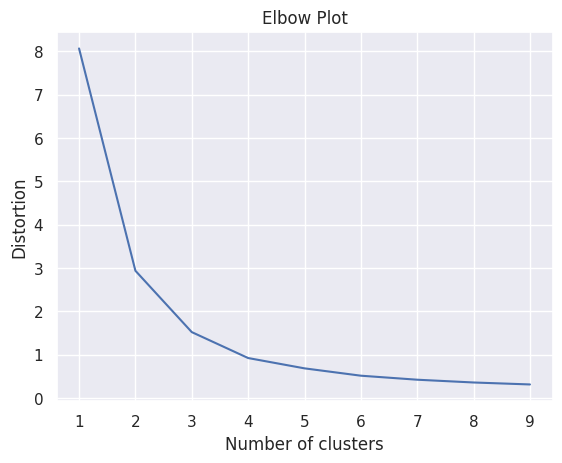
\includegraphics[width=\textwidth]{figures/tskmeans_elbow_b.png}
        \caption{Magnetic Field ($B$).}
        \label{fig:elbow_b}
    \end{subfigure}
    \hfill
    \begin{subfigure}[h]{0.48\textwidth}
        \centering
        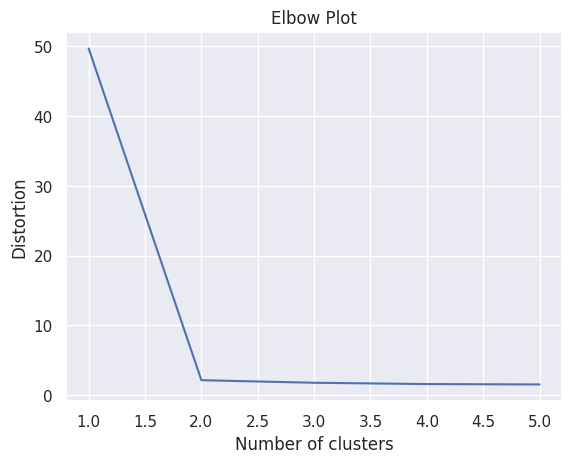
\includegraphics[width=\textwidth]{figures/tskmeans_elbow_alpha.png}
        \caption{Flux-tube inclination ($\alpha$).}
        \label{fig:elbow_alpha}
    \end{subfigure}
\end{figure}

\begin{table}[h]
    \caption[Validity Scores for TimeSeriesKmeans]{Validity metrics for different TimeSeriesKMeans models obtained by varying the number of clusters.}
    \begin{subtable}[h]{0.48\textwidth}
        \centering
        \begin{tabular}{@{}cccc@{}}
            \toprule
            \textbf{K} & \textbf{S score} & \textbf{DB} & \textbf{CH} \\ \midrule
            2          & 0.524               & 0.669                   & 20376                  \\
            3          & 0.511               & 0.628                   & 25585                  \\
            4          & 0.498               & 0.606                   & 30677                  \\
            5          & 0.458               & 0.648                   & 31995                  \\
            6          & 0.449               & 0.671                   & 34394                  \\
            7          & 0.431               & 0.695                   & 35462                  \\
            8          & 0.422               & 0.712                   & 36070                  \\
            9          & 0.403               & 0.738                   & 36368                  \\ \bottomrule
        \end{tabular}
        \caption{Magnetic Field ($B$)}
        \label{tab:tskmeans_b}
    \end{subtable}
    \hfill
    \begin{subtable}[h]{0.48\textwidth}
        \centering
        \begin{tabular}{@{}cccc@{}}
            \toprule
            \textbf{K} & \textbf{S score} & \textbf{DB} & \textbf{CH} \\ \midrule
            2          & 0.865               & 0.190                   & 263222                 \\
            3          & 0.499               & 1.078                   & 160481                 \\
            4          & 0.493               & 1.089                   & 120114                 \\
            5          & 0.463               & 1.123                   & 93537                  \\
            6          & 0.480               & 1.104                   & 82431                  \\
            7          & 0.259               & 1.312                   & 82038                  \\
            8          & 0.257               & 1.306                   & 76633                  \\
            9          & 0.252               & 1.374                   & 70313                  \\ \bottomrule
            \end{tabular}
        \caption{Flux-tube inclination ($\alpha$)}
        \label{tab:tskmeans_alpha}
    \end{subtable}
\end{table}


The elbow test for the magnetic field variable can be seen in Figure \ref{fig:elbow_b}. From this plot, it can be seen that the elbow is at $k=4$, which indicates that the optimal number of clusters is 4. However, this is not a clear elbow, as the curve is not smooth and the elbow is not very pronounced. This indicates that the optimal number of clusters is not very clear and that the results might not be very good.

To get a more precise number of clusters the validity metrics discussed in Section \ref{sec:validity_measures} were calculated for different KMeans models obtained by varying the number of clusters. The results of these tests can be seen in Table \ref{tab:tskmeans_b}. From the first three entries, it can be seen that the highest silhouette score is obtained with $K=2$, but the lowest Davies-Bouldin index is obtained with $k=4$, which also has the highest Calinski-Harabasz index of the three. This can serve as a possible indication that the correct number of clusters for this variable is 4.

Following the same procedure as for the magnetic field, an elbow test was conducted on the flux tube inclination variable, $\alpha$. The results of this test can be seen in Figure \ref{fig:elbow_alpha}. In contrast with the results of the previous test, this elbow is much clearer, with the elbow being at $k=2$. This indicates that the optimal number of clusters is 2.

The validity metrics (table \ref{tab:tskmeans_alpha}) also provide a clear indication that the correct number of clusters for this variable is 2, with the highest Silhouette and Calinski-Harabasz scores being obtained with $k=2$. The Davies-Bouldin index is also the lowest for this value.


\subsection{SOM}\label{sec:som_experiments}
Following the experiments with TimeSeriesKmeans, the SOM algorithm was tested, which is also seen as a useful method for clustering high-dimension data. This algorithm was tested on the same variables as the previous algorithm, $B$ and $\alpha$. The elbow tests for these variables can be seen in Figure \ref{fig:som_elbow}. From these plots, it can be seen that the elbow for the magnetic field variable is at $k=4$, while the elbow for the flux tube inclination variable is at $k=2$. This indicates that the optimal number of clusters for the magnetic field variable is 4, while the optimal number of clusters for the flux tube inclination variable is 2.

\section{Results}\label{sec:clustering_results}
